\section{The DDPM noise space}
\label{method}

% Given an input image x and a target text which describes
% the desired edit, our goal is to edit the image in a way that
% satisfies the given text, while preserving a maximal amount
% of detail from x (e.g., small details in the background and
% the identity of the object within the image).


% Bottom row: the right image is the originally generated image. Changing the Zs, while keeping the rest untouched, resulted in different generated images, depending on which steps they were changed. We can see that changing the Zs at the beginning of the generative process (images on the left), results in a very different image from the original one while changing the Zs toward the end of the process (images on the right) changes only the fine details from the original one.

% -- Katherine Crowson. Clip-guided diffusion. 2022. URL https://github.com/afiaka87/
% -- Since methods that require model finetuning or prompt tuning [6, 11, 25] can be combined with EDICT, we view them as complementary to, rather than competitive with, EDICT,
% and do not perform a direct comparison with them. We quantitatively compare visual metrics of edits
% }



Here we focus on the DDPM sampling scheme, which is applicable in both pixel space~\cite{Ho20} and latent space~\cite{Rombach22}. %In the latter case, a pre-trained decoder is applied to the generated output to recover an image. 
DDPM draws samples by attempting to reverse a diffusion process that gradually turns a clean image $x_0$ into white Gaussian noise,
\begin{equation}
\label{eq:xt_from_xtm1}
x_t = \sqrt{1-\beta_t} x_{t-1} + \sqrt{\beta_t}\, n_t,\quad t=1,\ldots,T,
\end{equation}
where $\{n_t\}$ are iid standard normal vectors and $\{\beta_t\}$ is some variance schedule. The forward process (\ref{eq:xt_from_xtm1}) can be equivalently expressed as
\begin{equation}
\label{eq:xt_from_x0}
x_t = \sqrt{\bar\alpha_t} x_0 + \sqrt{1-\bar\alpha_t}\, \epsilon_t,
\end{equation}
where $\alpha_t=1-\beta_t$, $\bar{\alpha}_t=\prod_{s=1}^t\alpha_s$, and $\epsilon_t\sim\mathcal{N}(0,\boldsymbol{I})$. It is important to note that in the representation \eqref{eq:xt_from_x0}, the vectors $\{\epsilon_t\}$ are \emph{not independent}. This is because each $\epsilon_t$ corresponds to the accumulation of the noises $n_1,\ldots,n_t$, so that $\epsilon_t$ and $\epsilon_{t-1}$ are highly correlated for all~$t$. This fact is irrelevant for the training process, %which is only affected by the joint distributions of the pairs $(\epsilon_t,x_0)$ and 
which is not affected by the joint distribution of $\epsilon_t$'s across different timesteps, but it is important for our discussion below.

The generative (reverse) diffusion process starts from a random noise vector $x_T \sim \mathcal{N}(0,\mathbf{I})$ and iteratively denoises it using the recursion %At each step $t=\{T,T-1,...,1\}$ the noisy signal $x_t$ is denoised to $x_{t-1}$ by the following relation
\begin{equation}
\label{eq:diffusion}
    x_{t-1} = \hat\mu_t(x_t) + \sigma_t z_t,\quad t=T,\ldots,1,
\end{equation}
where $\{z_t\}$ are iid standard normal vectors, and% $z_t \sim \mathcal{N}(0,\mathbf{I})$, and
\begin{align}
\label{eq:PD}
\hat\mu_t(x_t) = 
\sqrt{\bar \alpha_{t-1}} P(f_t(x_t)) + D(f_t(x_t)).
\end{align}
Here, $f_t$ is a neural network that is trained to predict  $\epsilon_t$ from $x_t$, $P(f_t(x_t))=(x_t-\sqrt{1-\bar \alpha_{t}}f_t(x_t))/\sqrt{\bar \alpha_{t}}$ is the predicted $x_0$, and $D(f_t(x_t))=\sqrt{1-\bar \alpha_{t-1}-\sigma_t^2} f_t(x_t)$ is a direction pointing to $x_t$. 
%\begin{align}
%\label{eq:diffusion}
%\hat\mu(x_t,t) = 
%\sqrt{\bar \alpha_{t-1}} &\underbrace{\biggl(\dfrac{x_t-\sqrt{1-\bar \alpha_{t}}f(x_t,t)}{\sqrt{\bar \alpha_{t}}}\biggl)}_\text{``predicted $x_0$''} + \nonumber\\
%&\underbrace{\sqrt{1-\bar \alpha_{t-1}-\sigma_t^2} f(x_t,t)}_\text{``direction pointing to $x_t$''}
%\end{align}
The variance schedule is taken to be $\sigma_t=\eta \beta_t (1-\bar{\alpha}_{t-1})/(1-\bar{\alpha}_t)$, where $\eta\in[0,1]$.
%Equation~\ref{eq:diffusion} is the general DDIM sampling. Different choices of $\eta$ values result in different generative processes. 
The case $\eta=1$ corresponds to the original DDPM work, and $\eta= 0$ corresponds to the deterministic DDIM scheme.

This generative process can be conditioned on text~\cite{Rombach22} or class~\cite{Ho21} by using a neural network $f$ that has been trained conditioned on those inputs. Alternatively, conditioning can be achieved through guided diffusion~\cite{Prafulla21,avrahami22}, which requires utilizing a pre-trained classifier or CLIP model during the generative process.

% \begin{equation}
% X_t = \sqrt{\bar\alpha_t} X_0 + \sqrt{1-\bar\alpha_t} \epsilon
% \setlength{\abovedisplayskip}{0.5pt}
% \setlength{\belowdisplayskip}{0.5pt}
% \end{equation}
%We unfold Equation~\ref{eq:diffusion}, and denote the generative process to be $D(x_T,\{z_t\}_{{t=1}}^T)$, with $T+1$ inputs sampled from a Gaussian distribution. 
% The evidence for this can be shown in Figure~\ref{fig:unfold}.





The vectors $\{x_T,z_T,\ldots,z_1\}$ uniquely determine the image $x_0$ generated by the process \eqref{eq:diffusion} (but not vice versa). We therefore regard them as the latent code of the model (see Fig.~\ref{fig:unfold}). Here, we are interested in the inverse direction. Namely, given a real image $x_0$, we would like to extract noise vectors that, if used in \eqref{eq:diffusion}, would generate $x_0$. We refer to such noise vectors as consistent with $x_0$. Our method, explained next, works with any $\eta\in(0,1]$.

\subsection{Edit friendly inversion}

% generates a new image. We denote the entire generative process with its $T+1$ inputs $D(X_T,\{z_t\}_{{t=1}}^T)$ or $D(X_T,\{z_t\}_{{t=1}}^T,c)$ in case of unconditional and conditional models respectively.
It is instructive to note that \emph{any} sequence of $T+1$ images $x_0,\ldots,x_T$, in which $x_0$ is the real image, can be used to extract consistent noise maps by isolating $z_t$ from \eqref{eq:diffusion} as\footnote{Commonly, $z_1=0$ in DDPM, so that we run only over $t=T,\ldots,2$.} 
\begin{equation}
\label{eq:z_t}
z_t = \dfrac{x_{t-1} -\hat\mu_t(x_t)}{\sigma_t},\quad t=T,\ldots,1.
\end{equation}
% It is instructive to note that \emph{any} sequence of $T+1$ images $x_0,\ldots,x_T$, that starts with the real image $x_0$, can be used to extract consistent noise maps by isolating $z_t$ from \eqref{eq:diffusion} as\footnote{Commonly, $z_1=0$ in DDPM, so that we run only over $t=T,\ldots,2$.}% Therefore, there are only $T$ non-trivial noise maps to recover.}
However, unless such an auxiliary sequence of images is carefully constructed, they are likely to be far from the distribution of inputs on which the network $f_t(\cdot)$ was trained. In that case, fixing the so-extracted noise maps, $\{x_T,z_T,\ldots,z_1\}$, and changing the text condition, may lead to poor results.

What is a good way of constructing auxiliary images $x_1,\ldots,x_T$ for \eqref{eq:z_t} then? A naive approach is to draw them from a distribution that is similar to that underlying the generative process. Such an approach was pursued by~\cite{Wu22}. Specifically, they start by sampling  $x_T \sim \mathcal{N}(0,\mathbf{I})$. Then, for each $t=T,\ldots,1$ they isolate $\epsilon_t$ from \eqref{eq:xt_from_x0} using $x_t$ and the real $x_0$, substitute this $\epsilon_t$ for $f_t(x_t)$ in \eqref{eq:PD} to compute $\hat{\mu}_t(x_t)$, and use this $\hat{\mu}_t(x_t)$ in \eqref{eq:diffusion} to obtain $x_{t-1}$.

The noise maps extracted by this method are distributed similarly to those of the generative process. Unfortunately, they are not well suited for editing global structures. This is illustrated in Fig.~\ref{fig:cyclediffusion_vs_us} in the context of text guidance and in Fig.~\ref{fig:shifting_bird} in the context of shifts. The reason for this is that DDPM's native noise space is not edit-friendly in the first place. Namely, even if we take a model-generated image, for which we have the ``ground-truth'' noise maps, fixing them while changing the text prompt does not preserve the structure of the image (see Fig.~\ref{fig:generated_vs_us}).



\begin{figure}
% \vskip 0.2in
% \begin{center}
\centering
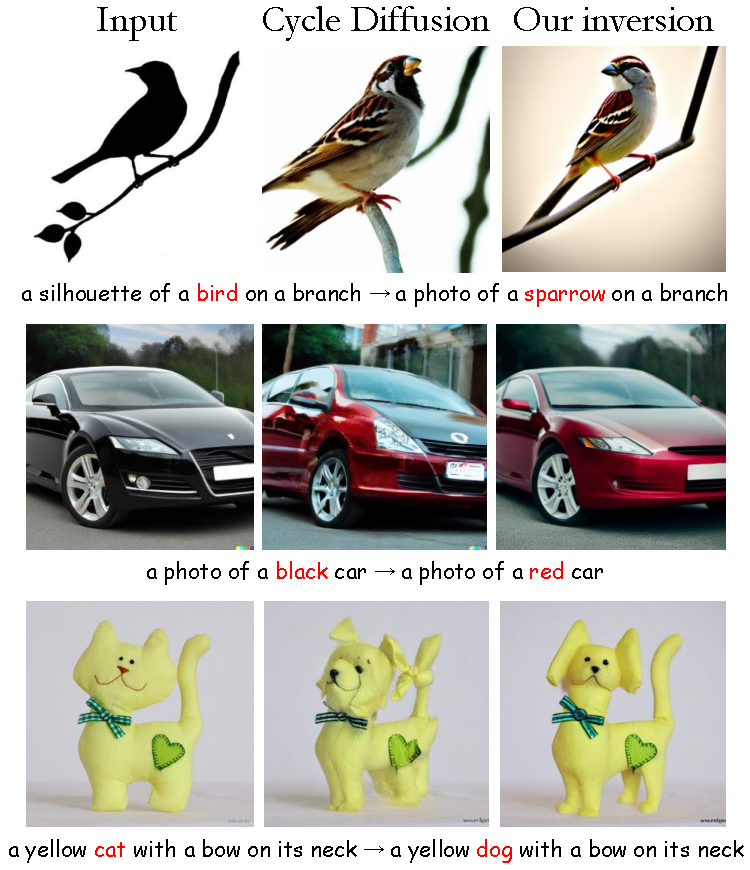
\includegraphics[width=0.94\columnwidth]{ICCV23_submission/figures/Cycle-Diffusion.pdf}
\caption{\textbf{DDPM inversion via CycleDiffusion vs.~our method.} CycleDiffusion's inversion~\cite{Wu22} extracts a sequence of noise maps $\{x_T,z_T,\ldots,z_1\}$ whose joint distribution is close to that used in regular sampling. However, fixing this latent code and replacing the text prompt fails to preserve the image structure. Our inversion deviates from the regular sampling distribution, but better encodes the image structure.}
\label{fig:cyclediffusion_vs_us}
% \end{center}
% \vskip -0.2in
\end{figure}


%The calculated $\{x_t\}_{{t=1}}^T$ have the same distribution as those from the generative process. Hence, $\{z_t\}_{{t=1}}^T$ that are extracted using these $\{z_t\}_{{t=1}}^T$ have Gaussian distribution.

%the inverse problem is defined as $E(X_0) = (x_T,\{z_t\}_{{t=1}}^T)$, extracting the start noise vectors as well as the noise vectors that are added at each timestep. Injecting them to $D$ results in reconstructing the input image $x_0$. We denote the extracted tuple $(x_T,\{z_t\}_{{t=1}}^T)$ as the latent space.

Interestingly, here we observe that constructing the auxiliary sequence $x_1,\ldots,x_T$ directly from $x_0$, and not via  (\ref{eq:xt_from_xtm1}), causes the image $x_0$ to be more strongly ``imprinted'' into the noise maps extracted from \eqref{eq:z_t}. 
% Here we propose to construct the auxiliary sequence $x_1,\ldots,x_T$ such that structures within the image $x_0$ would be more strongly ``imprinted'' into the noise maps extracted from \eqref{eq:z_t}. 
Specifically, we propose to construct them as
\begin{equation}
\label{eq:xt_from_x0_iid}
x_t = \sqrt{\bar\alpha_t} x_0 + \sqrt{1-\bar\alpha_t}\, \tilde{\epsilon}_t,\quad 1,\ldots,T,
\end{equation}
where $\tilde{\epsilon}_t\sim\mathcal{N}(0,\boldsymbol{I})$ are \emph{statistically independent}. Note that despite the superficial resemblance between \eqref{eq:xt_from_x0_iid} and \eqref{eq:xt_from_x0}, these equations describe fundamentally different stochastic processes. In \eqref{eq:xt_from_x0} every pair of consecutive $\epsilon_t$'s are highly correlated, while in \eqref{eq:xt_from_x0_iid} the $\tilde{\epsilon}_t$'s are independent. This implies that in our construction, $x_t$ and $x_{t-1}$ are typically farther away from each other than in \eqref{eq:xt_from_x0}, so that every $z_t$ extracted from \eqref{eq:z_t} has a higher variance than in the regular generative process. A pseudo-code of our method is provided in Alg.~\ref{alg:example}. 

%Our method is applied over the non-deterministic case of the DDIM ($\eta \neq 0$).

A few comments are in place regarding this inversion method. First, it reconstructs the input image up to machine precision, given that we compensate for accumulation of numerical errors (last row in Alg.~\ref{alg:example}), as we explain in the SM. Second, it is straightforward to use with any kind of diffusion process (\eg a conditional model~\cite{Ho2021Cascaded,Ho20,Rombach22}, guided-diffusion~\cite{Prafulla21},
classifier-free~\cite{Ho21}) by using the appropriate form for $\hat\mu_t(\cdot)$. Lastly, due to the randomness in \eqref{eq:xt_from_x0_iid}, we can obtain many different inversions. While each of them leads to perfect reconstruction, when used for editing they will lead to different variants of the edited image. This allows generating diversity in \eg text-based editing tasks, a feature not naturally available with DDIM inversion methods (see Fig.~\ref{fig:teaser} and SM).% and Sec.~\ref{sec:text}).


\begin{algorithm}[tb]
   \caption{Edit-friendly DDPM inversion}
   \label{alg:example}
\begin{algorithmic}
   \STATE {\bfseries Input:} real image $x_0$ 
   \STATE {\bfseries Output:} $\{x_T,z_T,\ldots,z_1\}$
   % \STATE $X = zeros(T,c,h,w)$
   \FOR{$t=1$ {\bfseries to} $T$}
   \STATE $\tilde{\epsilon} \sim \mathcal{N}(0,\,1)$
   \STATE $x_t \leftarrow \sqrt{\bar{\alpha_t}} x_0 + \sqrt{1-\bar{\alpha_t}} \tilde{\epsilon}$
   \ENDFOR
   \FOR{$t=T$ {\bfseries to} $1$}
   % \STATE $\hat \epsilon, \sigma_t = \hat\mu(x_{t+1},t)$
   \STATE $z_t \leftarrow (x_{t-1} -\hat\mu_t(x_{t})) / \sigma_t $   
   \STATE $x_{t-1} \leftarrow \hat\mu_t(x_{t})+\sigma_t z_t$ \quad // to avoid error accumulation
   %\STATE $x_t = \hat x_t$ 
   \ENDFOR
   \STATE {\bfseries Return:} $\{x_T,z_T,\ldots,z_1\}$
\end{algorithmic}
\end{algorithm}



\subsection{Properties of the edit-friendly noise space}
\label{sec:properties}
% HIRTUT
%Notice that without any restrictions, there are an infinite number of latent space $(x_T,\{z_t\}_{t=1}^T)$ that build exactly the input image, i.e.: $D(x_T,\{z_t\}_{t=1}^T) = x_0$. This includes Wu et al.~\cite{Wu22} that suggests using Equation~\ref{eq:diffusion} to calculate $\{x_t\}_{t=1}^T$ in the first step of the latent space extraction. In the case of model-generated images, the native $\{z_t\}_{t=1}^T$ that reconstruct the image are already supplied. Nevertheless, not all latent space produces meaningful results when they are further used for editing

    We now explore the properties of our edit-friendly noise space and compare it to the native DDPM noise space. We start with a 2D illustration, depicted in Fig.~\ref{fig:statistics_2d}. Here, we use a diffusion model designed to sample from $\mathcal{N}( \begin{psmallmatrix}10\\10\end{psmallmatrix},\mathbf{I})$. The top-left pane shows a regular DDPM process with $40$ inference steps. It starts from $x_T \sim \mathcal{N}(\begin{psmallmatrix}0\\0\end{psmallmatrix},\mathbf{I})$ (black dot at the bottom left), and generates a sequence $\{x_t\}$ (green dots) that ends in $x_0$ (black dot at the top right). Each step is broken down to the deterministic drift $\hat\mu_t (x_t)$ (blue arrow) and the noise vector $z_t$ (red arrow). On the top-right pane, we show a similar visualization, but for our latent space. Specifically, here we compute the sequences $\{x_t\}$ and $\{z_t\}$ using Alg.~\ref{alg:example} for some given $x_0\sim \mathcal{N}(\begin{psmallmatrix}10\\10\end{psmallmatrix},\mathbf{I})$. As can be seen, in our case, the noise perturbations $\{z_t\}$ are larger. This property comes from our construction of $x_t$, which are typically farther away from one another than in \eqref{eq:xt_from_x0}. How can the red arrows be longer and still form a trajectory from the origin to the blue cloud? Close inspection reveals that the angles between consecutive noise vectors tend to be obtuse. In other words, our noise vectors are (negatively) correlated across consecutive times. This can also be seen from the two plots in the bottom row, which depict the histograms of angles between consecutive noise vectors for the regular sampling process and for ours. In the former case, the angle distribution is uniform, and in the latter it has a peak at $180^\circ$. 

\begin{figure}
% \captionsetup[subfigure]{labelformat=empty}
\begin{center}
%\begin{subfigure}{}
%\centering
\hspace{0.45cm} Regular dynamics \hspace{1.1cm} Edit friendly dynamics\\
\hspace{0.2cm}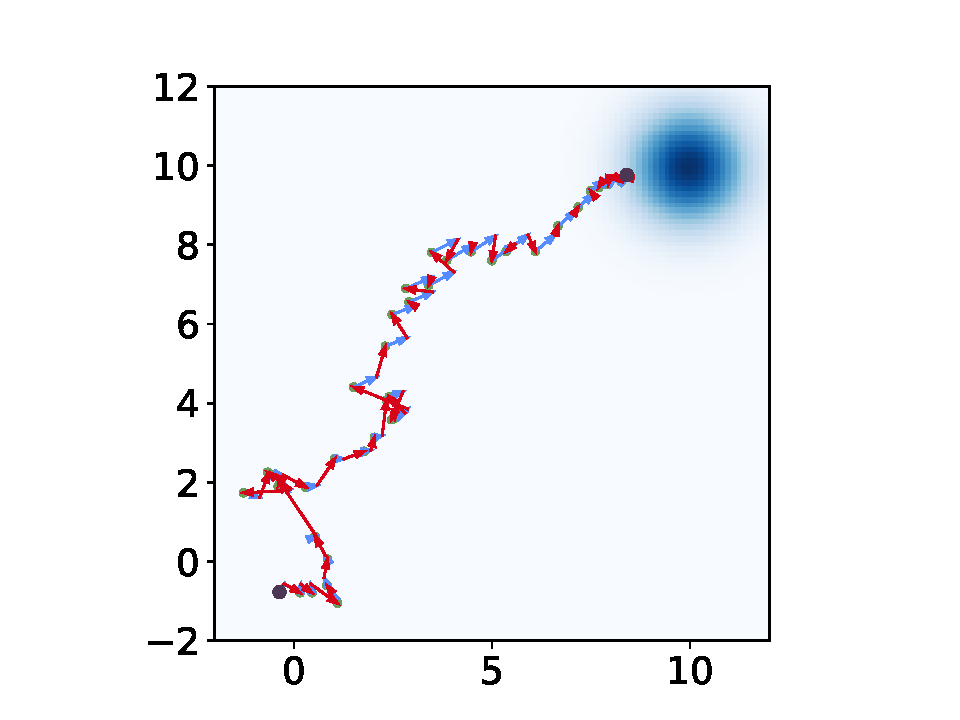
\includegraphics[width=0.47\columnwidth, trim={2.2cm 0cm 2.2cm 1.2cm},clip]{ICCV23_submission/figures/native_path.pdf}
% \caption{Test subfigure 2}
%\end{subfigure}%
%\begin{subfigure}{}
%\centering
\hspace{0.2cm}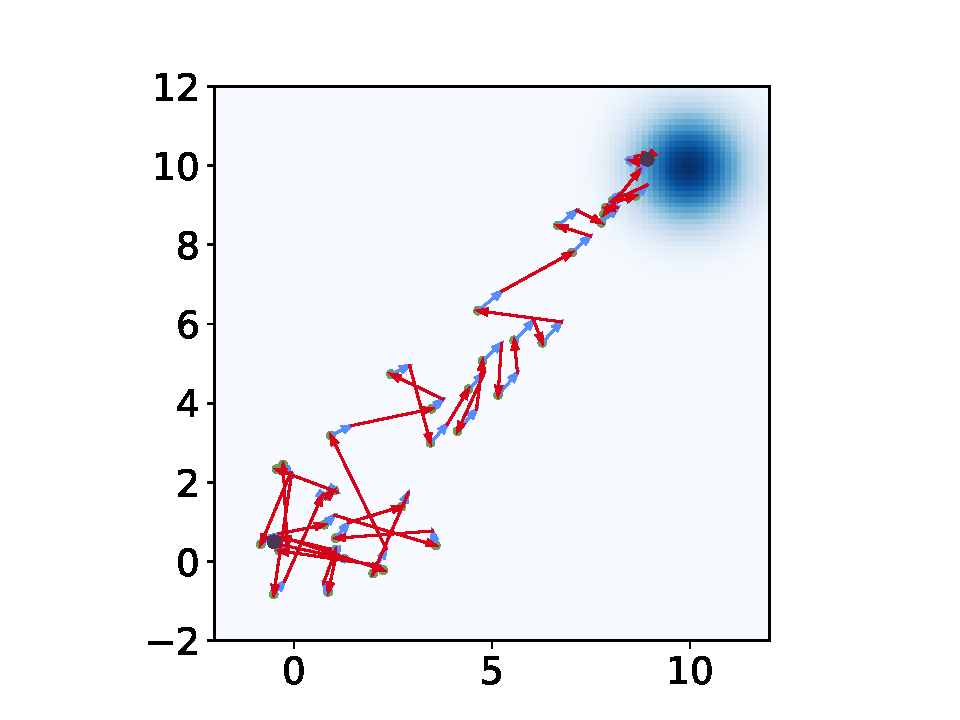
\includegraphics[width=0.47\columnwidth, trim={2.2cm 0cm 2.2cm 1.2cm},clip]{ICCV23_submission/figures/our_path.pdf}
% \caption{Test subfigure 2}
%\end{subfigure}%
%\begin{subfigure}{}
%\centering
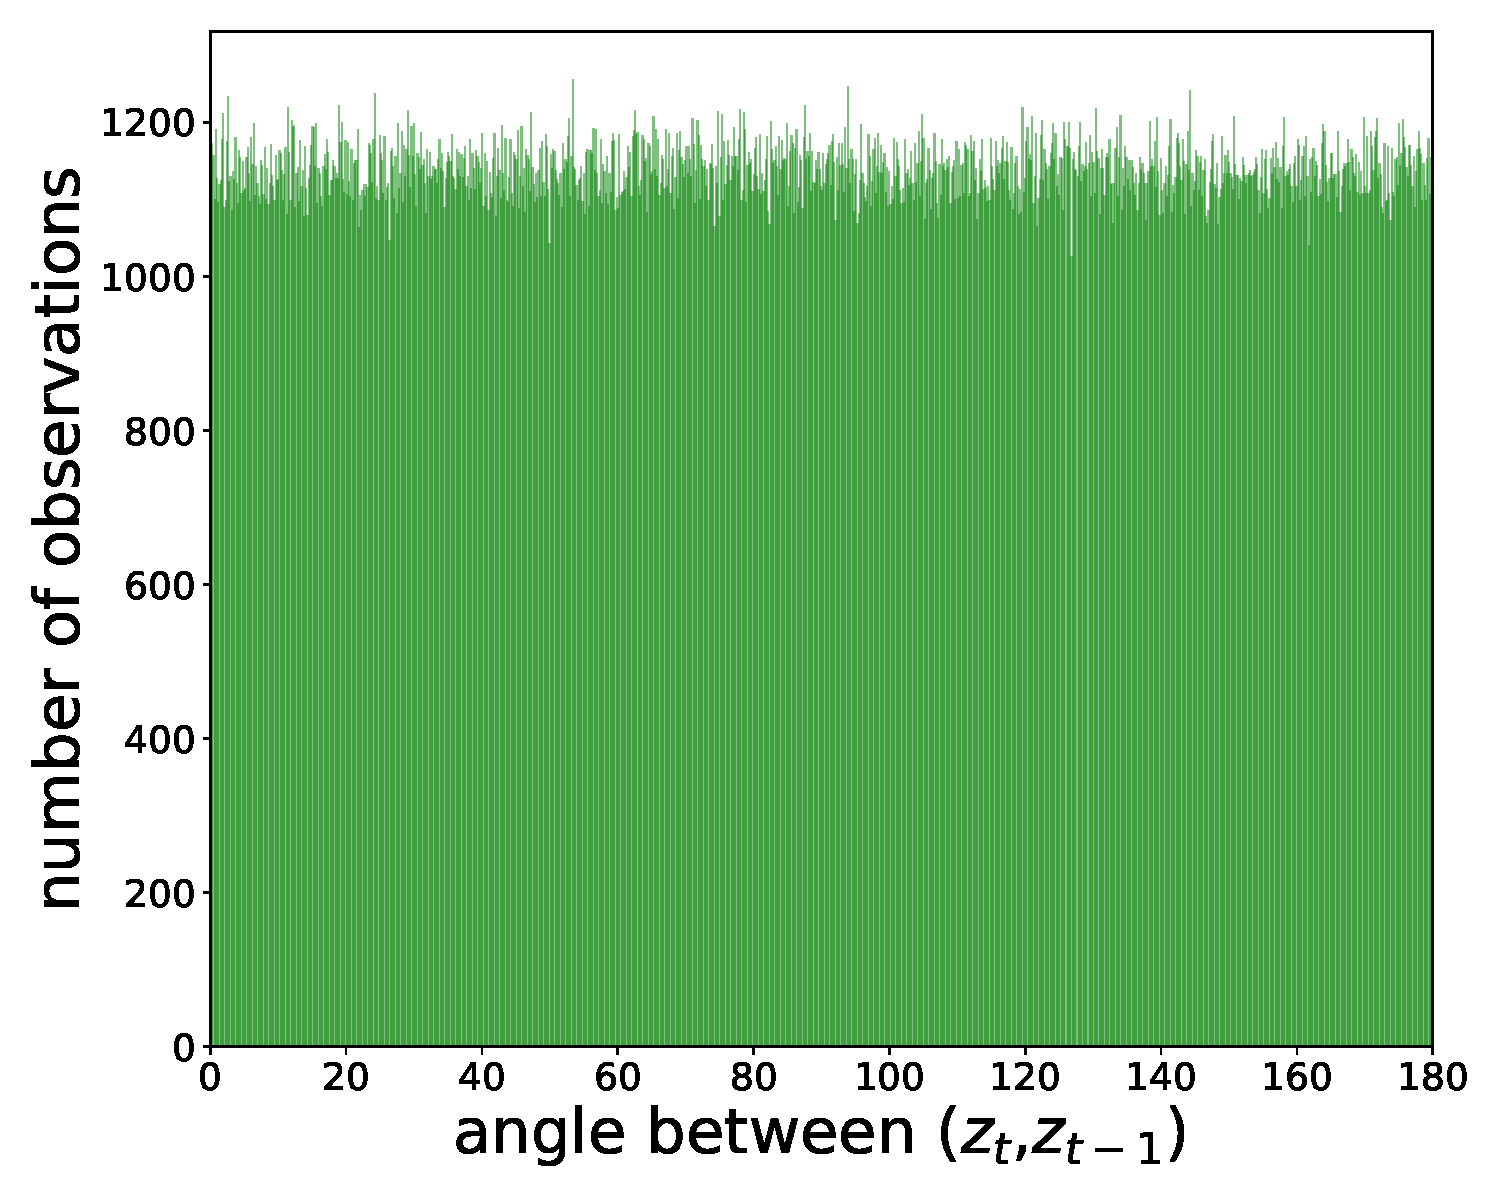
\includegraphics[width=0.49\columnwidth, trim={0cm 0cm 0cm 0.5cm},clip]{ICCV23_submission/figures/z_hist_reg.pdf}
% \caption{Test subfigure 2}
%\end{subfigure}%
%\begin{subfigure}{}
%\centering
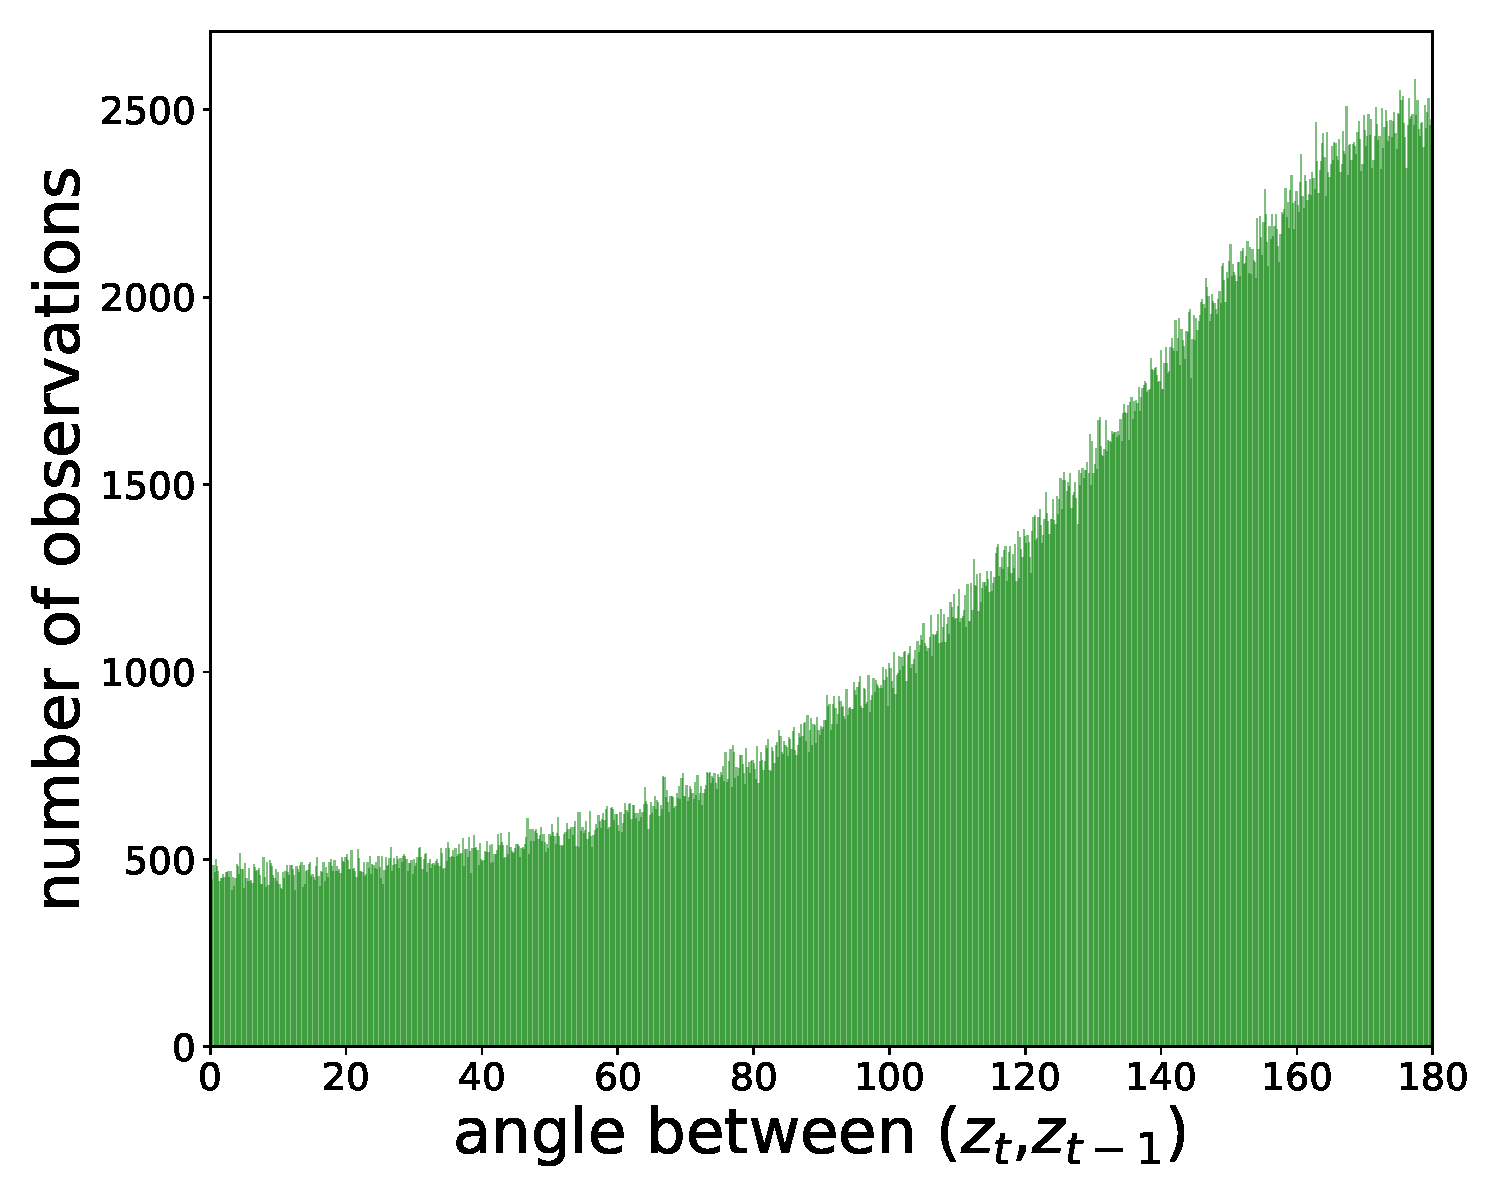
\includegraphics[width=0.49\columnwidth, trim={0cm 0cm 0cm 0.5cm},clip]{ICCV23_submission/figures/z_hist_ours.pdf}
% \caption{Test subfigure 2}
%\end{subfigure}%
\end{center}
\caption{\textbf{Regular vs.~edit-friendly diffusion.} In the regular generative process (top left), the noise vectors (red) are statistically independent across timesteps and thus the angle between consecutive vectors is uniformly distributed in $[0,180^\circ]$ (bottom left). In our dynamics (top right) the noise vectors have higher variances and are negatively correlated across consecutive times (bottom right).}
\label{fig:statistics_2d}
\end{figure}


The same qualitative behavior occurs in diffusion models for image generation. Figure~\ref{fig:statistics_images} shows the per-pixel variance of $z_t$ and correlation between $z_t$ and $z_{t-1}$ for sampling with 100 steps from an unconditional diffusion model trained on Imagenet. Here the statistics were calculated over 10 images drawn from the model. As in the 2D case, our noise vectors have higher variances and they exhibit negative correlations between consecutive steps. As we illustrate next, these larger variance noise vectors encode the structure of the input image more strongly, and are thus more suitable for editing. 

% As we illustrate next, these properties make our noise vectors more edit friendly. 

\begin{figure}
% \captionsetup[subfigure]{labelformat=empty}
%\begin{subfigure}{}
%\centering
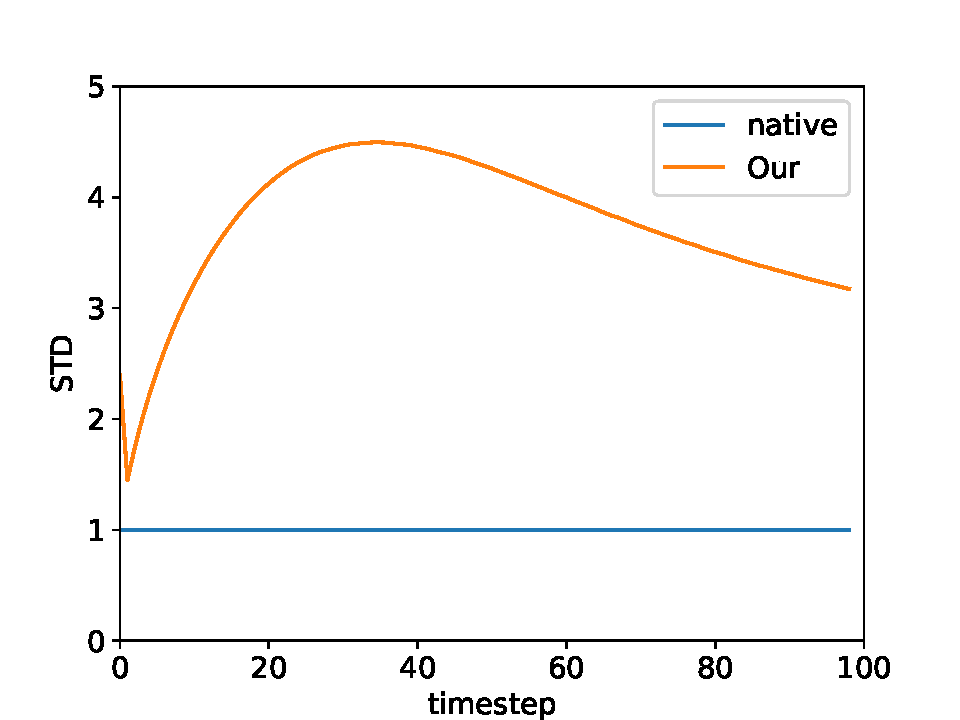
\includegraphics[scale=0.28, trim={0.8cm 0cm 1.2cm 1cm},clip]{ICCV23_submission/figures/std_no_cycle_native.pdf}
% \caption{Test subfigure 1}
%\end{subfigure}%
%\begin{subfigure}{}
%\centering
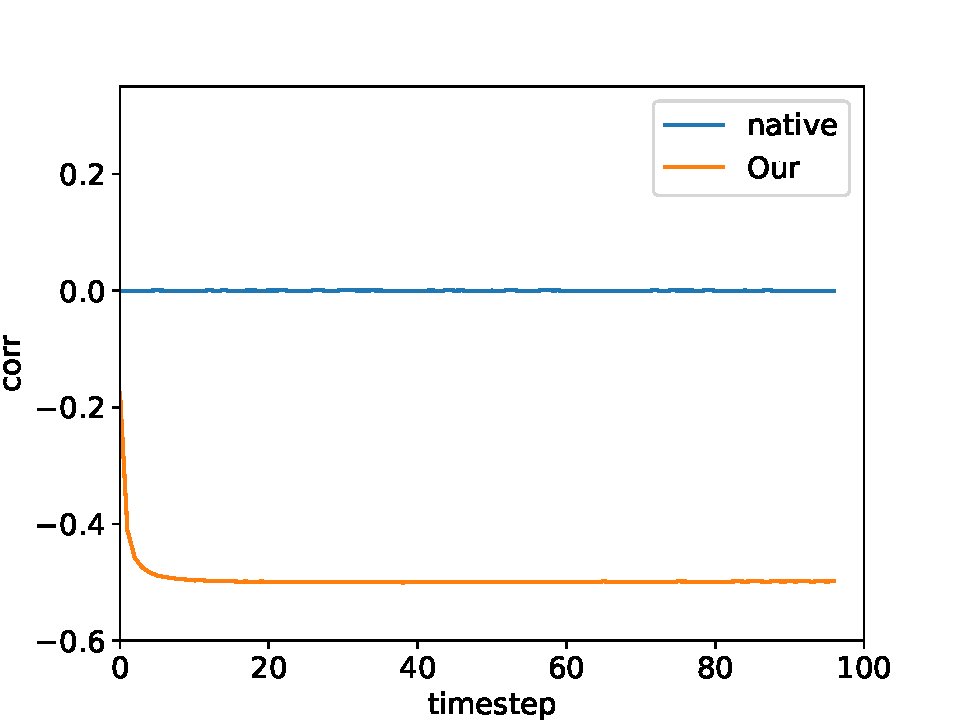
\includegraphics[scale=0.28, trim={0cm 0cm 1.2cm 1.2cm},clip]{ICCV23_submission/figures/corr_no_cycle_native.pdf}
% \caption{Test subfigure 2}
%\end{subfigure}%
%\begin{subfigure}{}
%\centering
%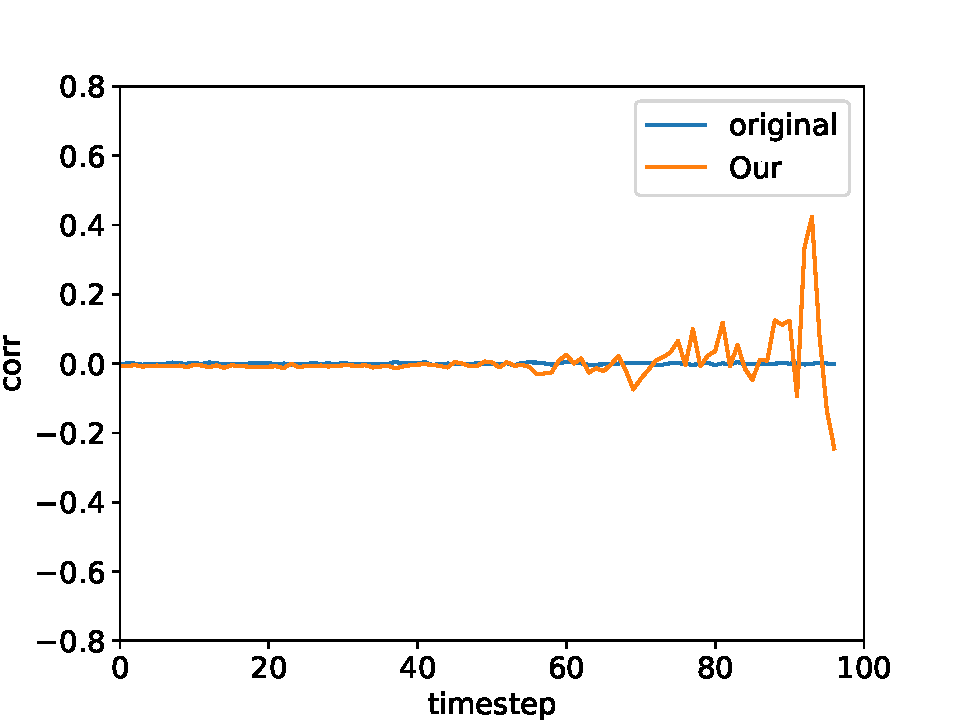
\includegraphics[width=0.33\textwidth]{ICCV23_submission/figures/corr_to_pred.pdf}
% \caption{Test subfigure 2}
%\end{subfigure}%
\caption{\textbf{Native vs.~edit friendly noise statistics.} Here we show the per-pixel standard deviations of $\{z_t\}$ and the per-pixel correlation between them for model-generated images.}
\label{fig:statistics_images}
\end{figure}


\begin{figure}
% \vskip 0.2in
% \begin{center}
\centering
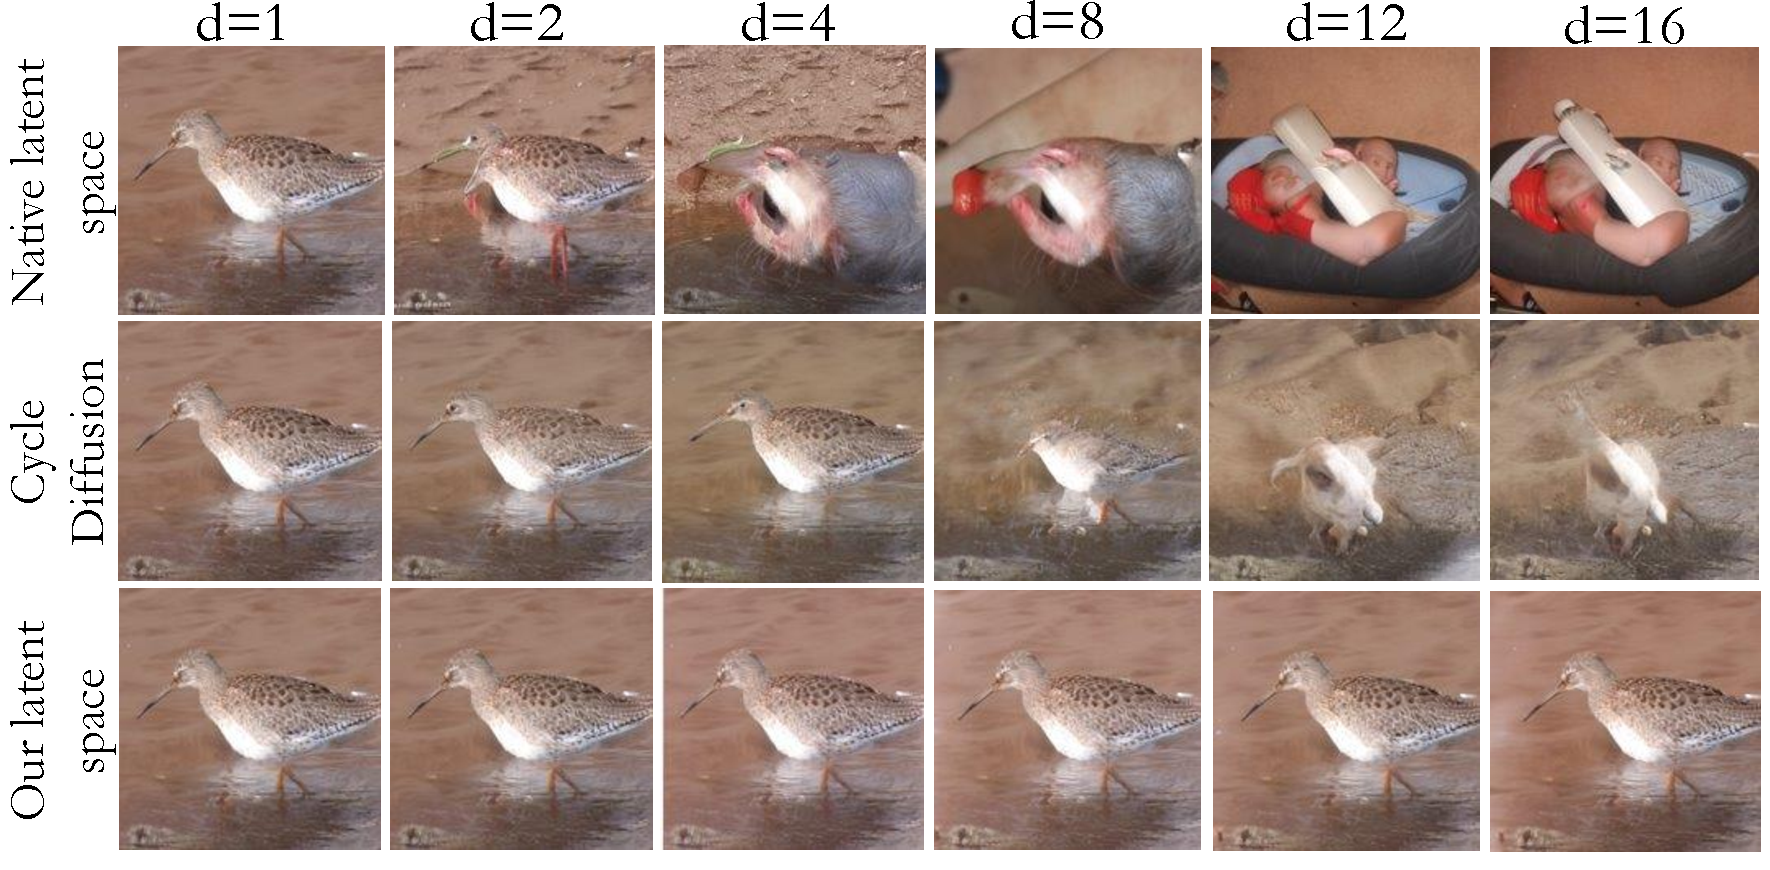
\includegraphics[width=\columnwidth]{ICCV23_submission/figures/shifting.pdf}
\caption{\textbf{Image shifting.} We shift to the right a $256 \times 256$ image generated by an unconditional model trained on ImageNet by $d=1\ldots16$ pixels. When shifting the native noise maps (top) or the ones extracted by CycleDiffusion \cite{Wu22} (middle) the structure is lost. With our latent space, the structure is preserved.}
\label{fig:shifting_bird}
% \end{center}
% \vskip -0.2in
\end{figure}

%\begin{figure}
% \vskip 0.2in
% \begin{center}
%\centering
%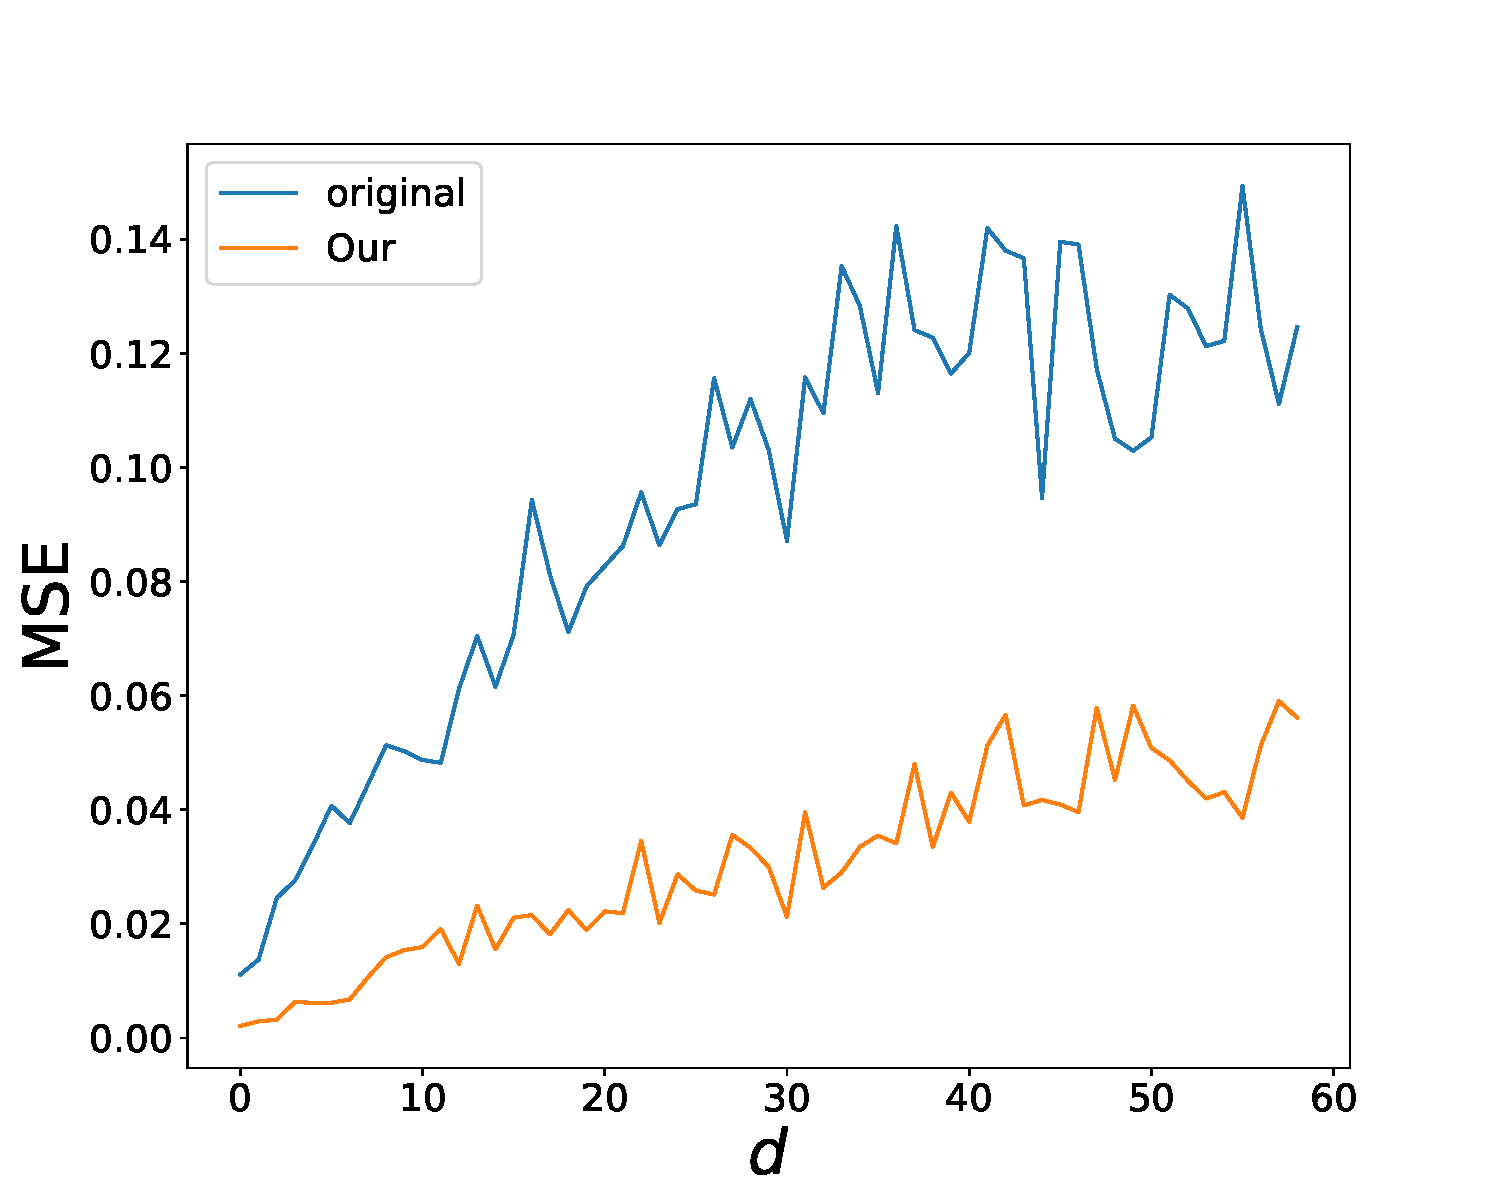
\includegraphics[width=0.7\columnwidth]{ICCV23_submission/figures/mse_shifting.pdf}
%\caption{\textbf{MSE in image shifting.} We plot the MSE (average over valid pixels of 20 generated images) between input images and ones obtained by shifting the noise maps by $d$ pixels. Our latent space is advantageous over the native one.}
%\label{fig:shifting_graph}
% \end{center}
% \vskip -0.2in
%\end{figure}



% Once $\{x_t\}_{t=1}^T$ created at the first step,  $\{z_t\}_{t=1}^T$ is easily extracted at the second step. Hence, the difference between the latent space editability is hidden in the first step. 

% Naively, we could follow Wu et al.~\cite{Wu22}, and use Equation~\ref{eq:diffusion} to calculate them. Having the real image, $x_0$, replacing the "predicted $x_0$" part with $x_0$ and $f(x_t,t)$ with $\big(\frac{x_t-\sqrt{\bar \alpha_t} x_0}{\sqrt{1-\bar \alpha_t}}\big)$. In this way, $\{x_t\}_{t=1}^T$ have the same properties as in they are calculated in the generative process. In cases of fake images, we could just use the original latent space for editing purposes.

% We claim that our extracted latent space is ideal for editing usage. As shown in Figure~\ref{fig:teaser} and Figure~\ref{fig:shifting_bird}, using the naive or the original (if have) latent space yields images deviating from the input one. Unlike Parmar et al.~\cite{Parmar23} that apply a DDIM inversion while requiring the start noise to be uncorrelated Gaussian white, we do not aim to extract noise vectors with statistical properties of Gaussian Noise.

% However, this latent space can be further used for editing the image. One can manipulate (Section~\ref{sec:manipulations}) the latent space before it is injected into the generative model or use different conditions in the generative model (Section~\ref{sec:text}).

% A different option is to integrate our inversion into existing editing methods, such as prompt-to-prompt~\cite{Hertz22} and plug-and-play~\cite{Narek22}, and provide them with the ability to work on real images, as described in Section~\ref{sec:p2p}.


% Our generated images show competitive results, without any further training.

% \subsubsection{Simple Image Manipulations}
% \label{sec:manipulations}
% In this section, we apply manipulations over the latent space in order to achieve image shifting, interpolation between images, and color changing. The new latent space is then used to create an edited image, i.e., fed into $D(x_T,\{z_t\}_{{t=1}}^T)$. Horizontal and vertical image flipping are shown in the appendix~\ref{}. This simple manipulation show how well the latent space behaves.


\vspace{-0.4cm}
\paragraph{Image shifting}
% \label{sec:shifting}
Intuitively, shifting an image should be possible by shifting all $T+1$ maps of the latent code. % Then, this new latent space is fed back into the generative model $D(x_T,\{z_t\}_{{t=1}}^T)$.
Figure~\ref{fig:shifting_bird} shows the result of shifting the latent code of a model-generated image by various amounts. As can be seen, shifting the native latent code (the one used to generate the image) leads to a complete loss of image structure. In contrast, shifting our edit-friendly code, results in minor degradation. Quantitative evaluation is provided in the SM.% in the supplementary material (SM). %Figure~\ref{fig:shifting_graph} compares the MSE incurred by the two methods. In both approaches, fidelity to the input image degrades as the translation $d$ is increased, but the edit-friendly approach significantly outperforms the native latent space. 

%It seems that although the original latent space of a generated image is available, it is better to ignore it and use our inversions to get an editable latent space. \inbar{Notice that in the case of producing several shifts as done in Figure~\ref{fig:shifting_bird}, we should use the same filled noise between the shifts in order to make a continuous sequence, i.e., the noise added in the first column in $d=1$ should be the same as the noise added in the second column in $d=2$. The first columns in $d=2$ will be drawn from Gaussian noise.}


% \subsubsection{inpainting}
% compare to RePaint.
% ~10 min for one image!!
% We proceed through the full reverse diffusion process, starting at the end time, at each step jumping back and forth a fixed number of time steps to progressively improve generation quality.
% Inpainting in imagenet - they mention they generate more images of dogs. Anyway, bad results using imagenet 256x256 unconditional model.
% % \begin{figure}
% % % \label{fig:reconstrcution}
% % \vskip 0.2in
% % % \begin{center}
% % 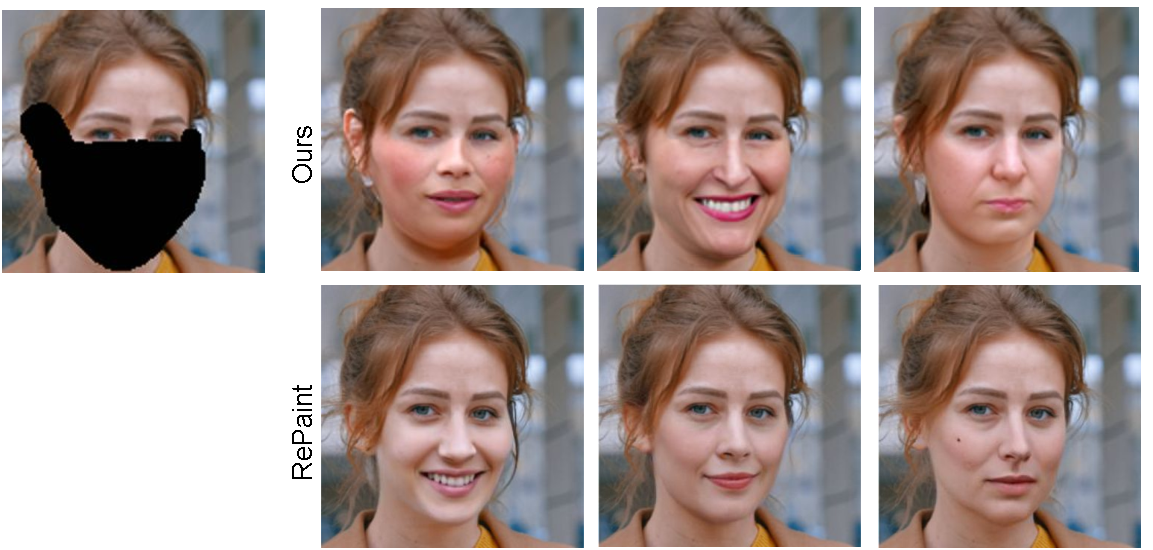
\includegraphics[width=\columnwidth]{figuers/inpainting.pdf}
% % \caption{Inpainting comparison.}
% % \label{fig:unfold}
% % % \end{center}
% % % \vskip -0.2in
% % \end{figure}



\vspace{-0.4cm}
\paragraph{Color manipulations}
% \label{sec:mask}
Our latent space also enables convenient manipulation of color. 
% Manipulating over the colors of an image can be done globally or locally, with a mask provided $M$.
% For example, changing the entire image to be more greenish or changing the sky from white to blue, respectively. Global change can be considered as a mask with a solid color.
Specifically, suppose we are given an input image $x_0$, a binary mask $B$, and a corresponding colored mask $M$. We start by constructing $\{x_1,\ldots,x_T\}$ and extracting $\{z_1,\ldots,z_T\}$ using \eqref{eq:xt_from_x0_iid} and \eqref{eq:z_t}, as before. Then, we modify the noise maps as
%We edit the latent space from a certain timestep $l$ to $0$. At each timestep $t=\{l..0\}$, the predicted input, $\hat X_0^t$, is calculated:
%\begin{equation}
%\label{eq:x0_from_xt}
%\setlength{\abovedisplayskip}{0.5pt}
%\setlength{\belowdisplayskip}{0.5pt}
%\hat x_0^t = \dfrac{x_t - \sqrt{1- \bar \alpha_t} f_t(x_t)}{\sqrt{\bar \alpha_t}}
%\setlength{\abovedisplayskip}{0.5pt}
%\setlength{\belowdisplayskip}{0.5pt}
%\end{equation}
%and update the latent space as follows:
\begin{equation}
\label{eq:zt_mask}
%\setlength{\abovedisplayskip}{0.5pt}
%\setlength{\belowdisplayskip}{0.5pt}
%z_t^{\text{edited}} = (1-B)\odot z_t + B\odot(z_t+s( M-P(f_t(x_t)))),
z_t^{\text{edited}} = z_t + s B\odot ( M-P(f_t(x_t))),
%\setlength{\abovedisplayskip}{0.5pt}
%\setlength{\belowdisplayskip}{0.5pt}
\end{equation}
with $P(f_t(x_t))$ from \eqref{eq:PD}, where $s$ is a parameter controlling the editing strength. We perform this modification over a range of timesteps $[T_1,T_2]$. Note that the term in parenthesis encodes the difference between the desired colors and the predicted clean image in each timestep. 
%This operation was also tested by SDEdit~\cite{Meng22}, by first multiplying the image with the mask, adding noise, and then denoise it through the stochastic differential equation (SDE) to increase its realism. SDEdit naturally finds a trade-off between realism and faithfulness: adding more noise and run the SDE for longer, the synthesized images are more realistic but less faithful. Similarly to SDEdit, we need to find from what timestep we start applying the mask on the latent space to obtain desirable and realistic images. However, their inference process might result in a deviation from the original image. 
Figure~\ref{fig:mask_color} illustrates the effect of this process in comparison to SDEdit, which suffers from an inherent tradeoff between fidelity to the input image and conformation to the desired edit. Our approach can achieve a strong editing effect without modifying textures (neither inside nor outside the mask). %Examples of global color changing can be found in Appendix~\ref{}.








%\section{Text-Guided Image Editing}
%\label{sec:text}

\vspace{-0.1cm}
\section{Text-Guided Image Editing} Our latent space can be utilized for text-driven image editing. 
\label{sec:text-guided}% where we generate an image that compiles with a target prompt while preserving the structure of the original real image. 
Suppose we are given a real image $x_0$, a text prompt describing it $p_{\text{src}}$, and a target text prompt $p_{\text{tar}}$. To modify the image according to these prompts, we extract the edit-friendly noise maps $\{x_T,z_T,\ldots,z_1\}$, while injecting $p_{\text{src}}$ to the denoiser. We then fix those noise maps and generate an image while injecting $p_{\text{tar}}$ to the denoiser. We run the generation process starting from timestep $T\!-\!T_{\text{skip}}$, where $T_{\text{skip}}$ is a parameter controlling the adherence to the input image.
Figures~\ref{fig:teaser},~\ref{fig:generated_vs_us},~\ref{fig:cyclediffusion_vs_us}, and \ref{fig:comparisons} show several text driven editing examples using this approach. As can be seen, this method nicely modifies semantics while preserving the structure of the image. In addition, it allows generating diverse outputs for any given edit (see Fig.~\ref{fig:teaser} and SM).
%~\ref{fig:variability1} and~\ref{fig:variability2} ).  %the text-driven editing ability in real images of our inversion as well as of existing methods with and without our inversion.
%\paragraph{Integrating into existing methods.}
We further illustrate the effect of using our inversion in combination with methods that rely on DDIM inversion (Figs. ~\ref{fig:teaser} and \ref{fig:zero-short-qualitative}). As can be seen, these methods often do not preserve fine textures, like fur, flowers, or leaves of a tree, and oftentimes also do not preserve the global structure of the objects. By integrating our inversion, structures and textures are better preserved.
% Figures~\ref{fig:teaser}, \ref{fig:comparisons} and \ref{fig:zero-short-qualitative} further illustrate the effect of using our inversion in combination with methods that rely on DDIM inversion. As can be seen, these methods often do not preserve fine textures, like fur, flowers, or leaves of a tree, and oftentimes also do not preserve the global structure of the objects. 

%Our extracted latent code can also be useful for methods that struggle with editing real images. The problematic part of existing methods is their poor reconstruction (not accurate, blurry, missing details, etc...). This drawback hurts the performance of the rest of the method since the details that are missing from the reconstruction, are not added back. 

\begin{figure}
\centering
\vspace{-0.05in}
\hspace{1in}

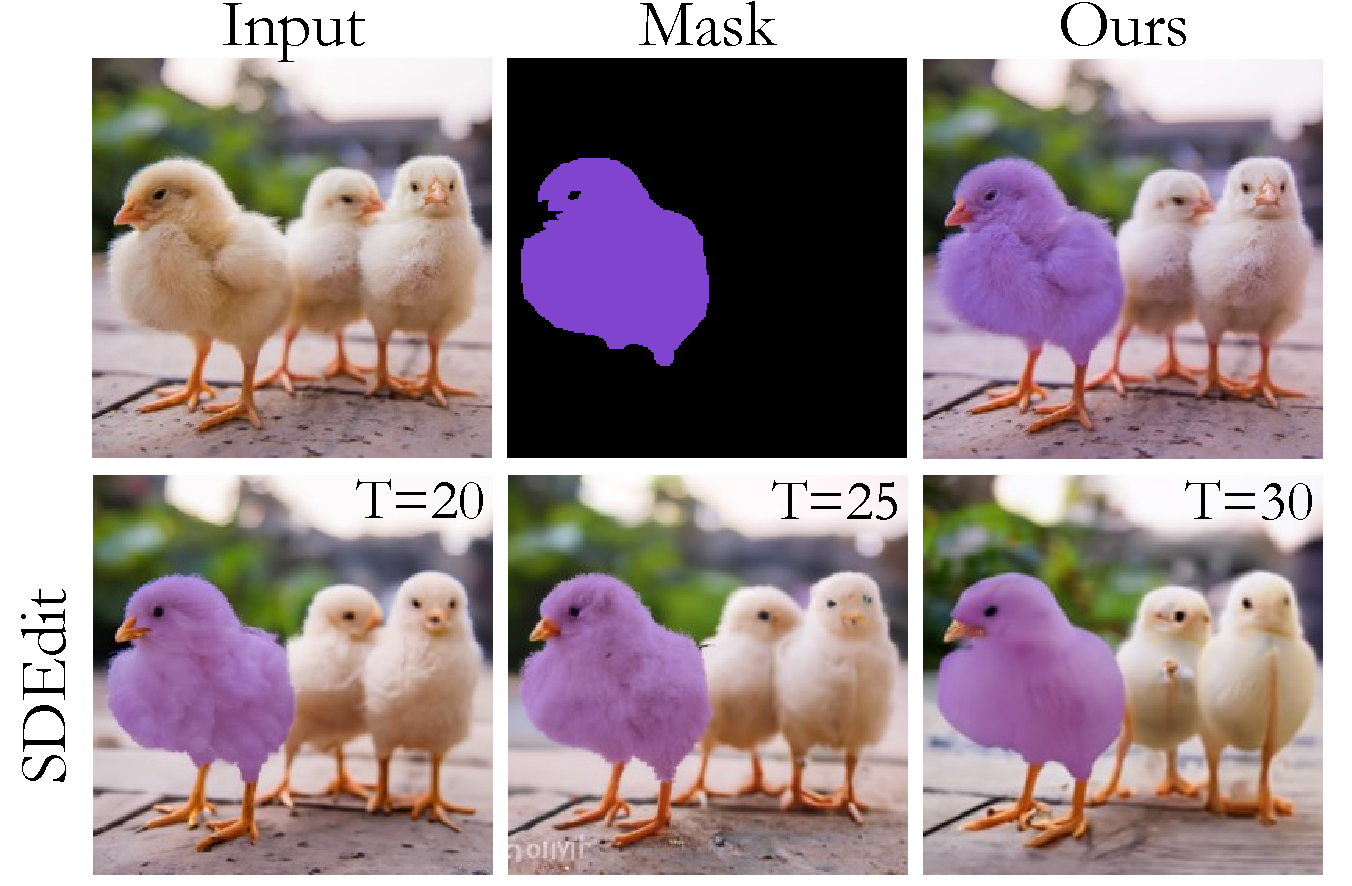
\includegraphics[width=0.9\columnwidth]{ICCV23_submission/figures/SDEdit.pdf}
\caption{\textbf{Color manipulation on a real image.} Our method (applied here from $T_2=70$ to $T_1=20$ with $s=0.05$) leads to a strong editing effect without modifying textures and structures. SDEdit, on the other hand, either does not integrate the mask well when using a small noise (left) or does not preserve structures when the noise is large (right). In both methods, we use an unconditional model trained on ImageNet with $100$ inference steps.} 
\label{fig:mask_color}
% \end{center}
% \vskip -0.2in
\end{figure}

%Figure~\ref{fig:comparisons} depicts the text-driven editing ability in real images of our inversion as well as of existing methods with and without our inversion.


% \begin{figure}
% % \vskip 0.2in
% % \begin{center}
% \includegraphics[width=\columnwidth]{ICCV23_submission/figures/text.png}
% \caption{Examples of editing real images with text. The first rows are the input images with the respective input prompt. Our results are presented in the second row, with the target text. These examples show our ability to make semantic changes to the foreground and the background of the image. We use stable diffusion for producing these results, expect for the snake image that is generated using CLIP guidance over the pixel space. \inbar{add more results to each example to show variety of images}}
% \label{fig:text}
% % \end{center}
% % \vskip -0.2in
% \end{figure}

% all below are based on ddim, so they produce only one output.
% compare to: p2p (prompt-2-prompt, DiffuseIT, Plug-and-Play, DiffuseDiff - no optimization over image.
% consider: DiffusionCLIP, Imagic,- with optimization


% \paragraph{Interpolations}
% % \label{sec:interpolations} 
% Given two images $x^0,x^1$, we extract their latent space, $D^1, D^2$ and interpolate them using spherical linear interpolation (slerp)~\cite{Ken85}.

% Figure~\ref{fig:interpolations} depicts interpolation results between two real images. The DDPM~\cite{Ho20} paper suggests interpolating the noisy versions of the images, at a certain $t$, then denoised it back in the generative process. There is a tradeoff between producing appealing results (larger $t$) and being faithful to the original images (smaller $t$). In the DDIM paper~\cite{Song21}, they first find $x_T$ of both images using the DDIM inversion and denoise back the interpolated starting noise. Our interpolation seems smoother with gradual changes in the facial attributes between the two endpoints. 
% % Although DiffusionAE~\cite{Preechakul22} suggest a learnable encoder for discovering high-level semantics, 

% \begin{figure}
% % \vskip 0.2in
% % \begin{center}
% \includegraphics[width=\columnwidth]{figures/interpolations.png}
% \caption{Interpolations between real images.}
% \label{fig:interpolations}
% % \end{center}
% % \vskip -0.2in
% \end{figure}
% \end{figure}

\begin{figure*}
% \vskip 0.2in
% \begin{center}
\centering
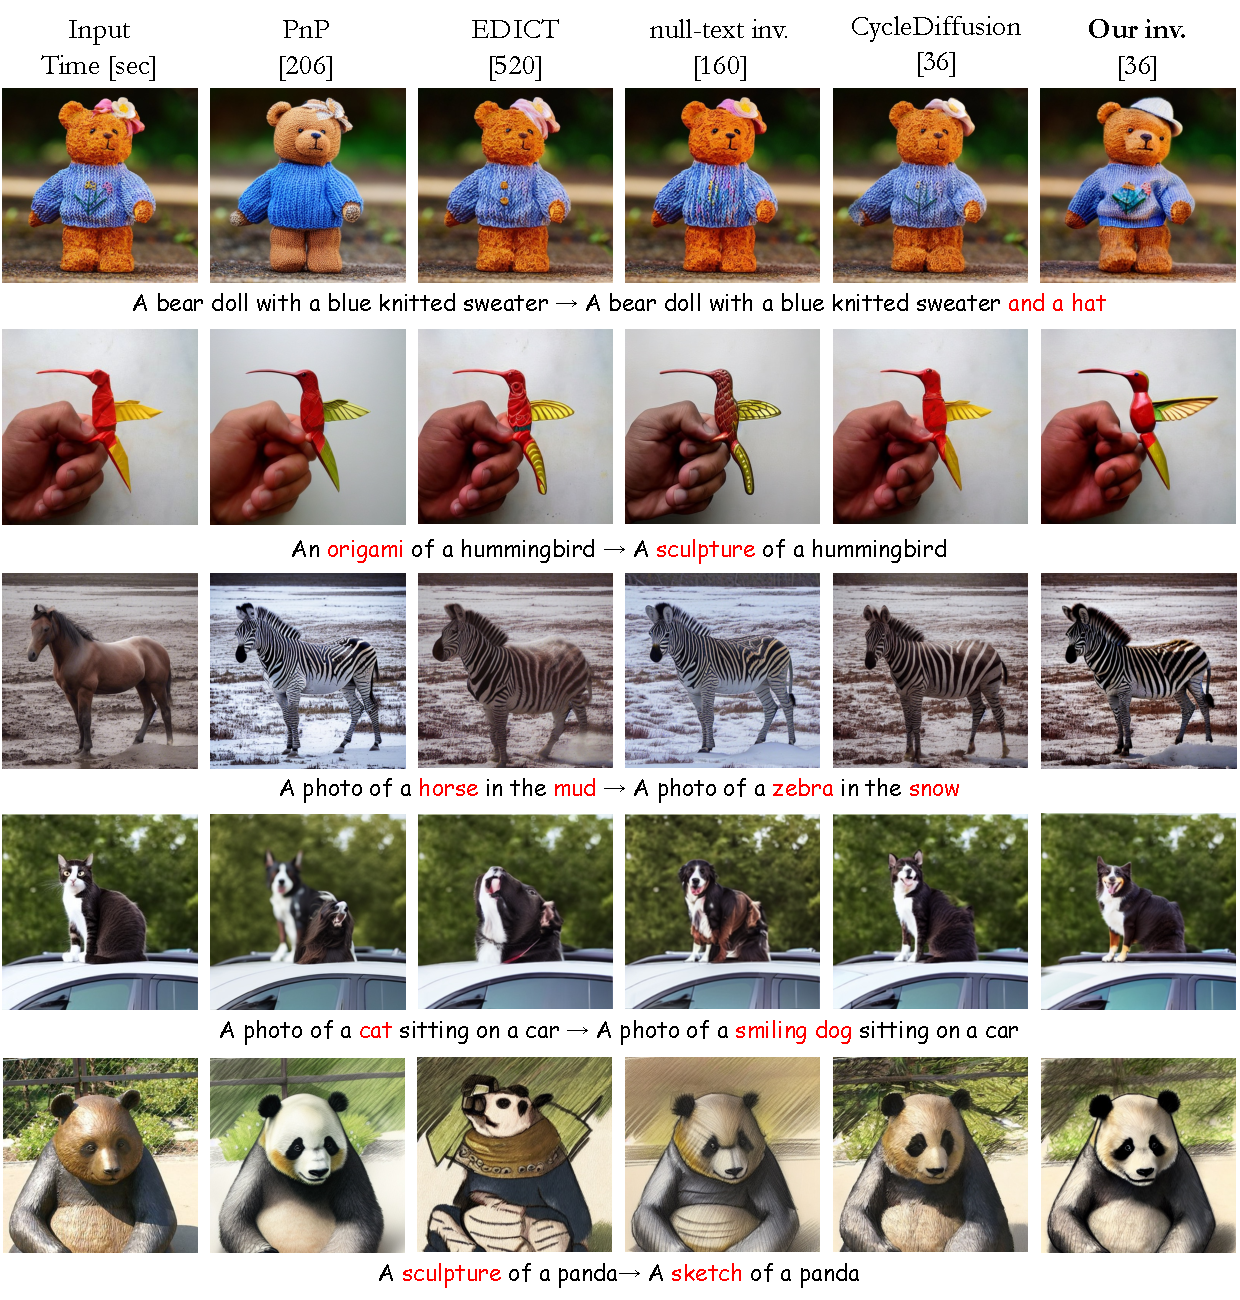
\includegraphics[width=0.8\textwidth]{ICCV23_submission/figures/comparisons_new.pdf}
\caption{\textbf{Comparisons.} We show results for editing of real images using all methods. Our approach maintains high fidelity to the input while conforming to the text prompt. The time taken to edit a single image is indicated within parentheses.}
\label{fig:comparisons}
% \end{center}
% \vskip -0.2in
\end{figure*}
